% ===========================================================================
\section{Uncertainty, and What Correlation Does to It}
\label{sec:uncertainty}
% ===========================================================================

Uncertainty is reported three ways: IPCC Approach~1 error propagation per sector, a pooled
Approach~2 Monte-Carlo simulation over every component in the inventory, and the same
simulation run again with the shared emission factors correlated. The third is the one with
a finding in it.

\subsection{Approach 1 and Approach 2 diverge, and the divergence is the finding}

Approach~1 combines each component's relative uncertainty in quadrature, treating correlated
components as summing linearly within their group before the squaring. Approach~2 accumulates
\num{100000} realisations of the national total---and it is a MIXTURE, not one
family: the waste and fugitives modules inject their own sector engines' persisted draws
(waste's ledger-true parameter rerun, whose fate identities hold in every realisation;
fugitives' bounded split-triangular), while every other module draws mean-preserving
lognormals. The draw files, their seeds and their SHA-256 hashes are in the release
manifest and \texttt{outputs/national\_uncertainty\_sources.csv}; the published run uses
ten times the sector default because the paper draws a conclusion from a difference
between two runs, and at \num{10000} draws the reported half-widths carry a Monte Carlo
standard error of the same order as that difference.

The two no longer agree closely, and the gap is the finding: \SI{10.9}{\percent} from
Approach~1 against \SI{11.72}{\percent} from
Approach~2 at the national level---quadrature is the analytic limit of the simulation
only under symmetric, independent, moderate uncertainties, and the injected engines are
deliberately none of those. The honest national statement is asymmetric,
$-\SI{10.3}{\percent}/+\SI{13.1}{\percent}$ about the median
(\texttt{rel\_down\_pct\_95}/\texttt{rel\_up\_pct\_95} in the published table), and a
single $\pm$ figure is printed only as a summary. The interval has two legitimate
reference points and they are not interchangeable: the same 2.5th--97.5th percentile
band (\SIrange{400.30}{504.97}{\mega\tonne}) read against the \emph{deterministic
reference} \SI{444.96}{\mega\tonne} is $-\SI{10.0}{\percent}/+\SI{13.5}{\percent}$,
because the deterministic total sits below the Monte-Carlo median
(\SI{446.52}{\mega\tonne}) and mean (\SI{448.14}{\mega\tonne})---the injected
engines are right-skewed, so re-running the accounting at parameter means does not land
on the distribution's centre. The recommended point estimate is the deterministic
reference \SI{444.96}{\mega\tonne} for accounting and comparison against other
inventories, and the median for any probabilistic statement; a reader attaching the
about-the-median percentages to the deterministic total is off by roughly a point in
each direction, which is why both readings are printed.

\textbf{And this interval is the narrowest statement the release makes, which is the wrong
one to borrow.} It is parametric and annual and national: it prices what the factors and
the activity data could be, and prices nothing about \emph{when} or \emph{where} the mass
was put. Both of those carry their own uncertainty, and neither is probabilistic---a
timing or placement bracket is a disagreement between two defensible readings of the same
evidence, and no probability attaches to a spread. So they are not summed into
$\sigma$. \texttt{outputs/pakemis\_joint\_uncertainty.csv} publishes the three components
separately, per category and per the \emph{resolution of the figure being read}, together
with an envelope---a bound, not a distribution---that widens the parametric interval by the
structural half-widths. A bracket only bites on the figure it can move: re-allocating a
category across districts does not change its national total, and re-profiling it across
months does not change its annual one. Nationally the bound widens from
$-\SI{10.37}{\percent}/+\SI{13.14}{\percent}$ annually to
$-\SI{23.3}{\percent}/+\SI{26.10}{\percent}$ for a district in a month. The four
resolutions form a lattice rather than a chain, because adding a month is not comparable to
adding a district. Timing is priced for seven categories of twenty (six on measured
dispersion, drawn in the ensemble) and placement for six,
and every row names what its envelope therefore omits; filling those cells with a weak
alternative would make the bound look rigorous and be worse.

Within a category the parametric error is perfectly correlated---one emission factor moves
every district and every month of it together---so intervals add \emph{linearly} across
districts and months and never in quadrature, and the gridded products deliberately carry no
per-cell interval that would invite the opposite. Across categories the simulation has
already measured the dependence, and adding the category intervals instead inflates the
national bound to $-\SI{22.0}{\percent}/+\SI{45.3}{\percent}$: not a conservative reading of
the evidence but a different and wrong one, asserting a coupling the correlation model
denies. \texttt{docs/uncertainty\_contract.md} states both rules and
\texttt{tests/test\_joint\_uncertainty.py} proves each by worked example.

\textbf{None of this is validation, and the two are registered separately.} A wide interval
that contains the truth and a narrow one that does not are indistinguishable from inside the
model, so \texttt{outputs/pakemis\_validation\_catalog.csv} records what has been compared
against what: \num{102} entries across the three properties an inventory can get wrong
independently---\num{50} magnitude, \num{20} timing, \num{32} geography---because a national
total agreeing with EDGAR does not validate a map and a satellite hotspot at a facility does
not validate a total. Every entry declares how independent its evidence was, and the answer
is usually not very: \num{20} carry \emph{large} independence, \num{45} only \emph{partial},
and \num{8} \emph{none} at all, meaning the comparison shares the activity data it is
testing (a further \num{10} are by-construction checks to which independence does not
apply). \num{11} rows are declared absences---a module and property with no independent
check, named rather than left blank, because a cell with nothing in it reads as a property
that was never at issue. Six absences in the register this catalogue replaced were found to
be false: the benchmarks had been scoring them all along and nobody had joined the two
registers, so the register understated what the project had actually checked.

Release 1.0.0rc33 unified that register with the frozen benchmark tasks into this one
catalogue (the older register itself was retired in 1.0.0rc35), in which every
validation asset declares its grain, its producer, and how it is wired into the build; a
validation product regenerated by the build itself must now be at least as new as the
build's first output or the build fails naming it, which on first contact exposed one
quality-cited check that nothing in the build produced and one whose producer depends on a
model held outside this repository. The catalogue's verdicts, previously six incompatible
vocabularies, are projected onto one closed set at read time. Its summary,
\texttt{outputs/pakemis\_validation\_scorecard.csv}, tabulates the full property-by-grain
space---magnitude, timing and geography at twelve grains from national to worksheet cell---
and \num{14} of its \num{36} cells are covered today; the remaining cells are written as
declared absences, so the scorecard is simultaneously the record of what has been validated
and the roadmap of what has not.

Three checks added this release each came back \emph{narrower} than they were built to be, and
the narrowing is recorded rather than rounded off. ERA5, on an independent reanalysis, tracks
the NASA POWER temperature behind the residential profile almost exactly in shape---correlation
\num{0.969} to \num{0.989} across five cities and \num{54} months---and disagrees on level by
a systematic \SIrange{3.2}{6.1}{\celsius}. That offset is definitional: the held grid carries
one value per cell per day and no metadata saying which value, so it validates the seasonal
\emph{timing} and cannot validate the degree-day series itself, degree days being a function of
level (\texttt{outputs/era5\_degree\_day\_crosscheck.csv}). APCMA's cement despatches, compiled
by the industry association rather than PBS, reproduce the QIM production shape to a mean
\SI{0.22}{} percentage points of the year over \num{60} months
(\texttt{apcma\_qim\_cement\_crosscheck.csv})---a real corroboration of the shape cement now
rides, on magnitudes that are deliberately not compared because despatches are sales. Its
feedstock corroborates it from a third direction: PBS limestone production tracks the QIM
cement shape to a mean \num{1.20} percentage points of the year over their six overlapping
years (\texttt{limestone\_qim\_cement\_crosscheck.csv}), once one flagged source anomaly is
set aside---November 2016 carries \SI{36.7}{\percent} of its year's limestone in a single
month, a defect in the mines-department series that is published and flagged rather than
dropped. That
parse is gated on three of the publication's own controls---each row's printed total, each
block's annual total, and agreement between the two pages that publish every year---and the
cells failing one are kept unrepaired with their raw text
(\texttt{apcma\_dispatch\_quarantine.csv}, \texttt{apcma\_dispatch\_parse\_summary.csv}). They
include a published digit-grouping error, an annual export total printed as \num{202989} where
its own twelve months sum to \num{2020569}, and small restatements between the two editions of
a year. And FAO's
rice calendar agrees with three of four provincial harvest windows
(\texttt{fao\_crop\_calendar\_crosscheck.csv}), which changed no provenance class, because the
methane profile rides the \emph{flooded} window and harvest is not one of its endpoints.

The divergence localises the assumption doing the work. The completed fugitives ledger gives
$\pm\SI{37.7}{\percent}$ under Approach~1
and $\pm\SI{19.0}{\percent}$ under the injected Approach~2---NARROWER, because the sector
engine's bounded split-triangular draws respect the published range endpoints where the
old lognormal surrogate's tails did not. Its
Monte-Carlo median is \SI{24.15}{\mega\tonne}, its mean
\SI{24.73}{\mega\tonne}---the sector engine's own quantities, reaching the national row
unconverted for the first time.

\subsection{The correlation question}

Six of the ten sector modules report \COtwo{} under an IPCC 1.A code, and they draw it
through the same default carbon-content factors. Transport (both its road and its off-road
categories), electricity generation, industrial fuel combustion, residential fuel, railways
and domestic aviation all take their fuel \COtwo{} factors from the same table entries with
the same published uncertainty ranges. The second case groups those components by the physical
factor each one uses: every row computed with the gas/diesel-oil carbon content draws one
realisation of it, every row computed with the natural-gas content draws another, and the two
are independent of each other. \textbf{It is a declared covariance sensitivity, not an
estimate of the true dependency structure}---see the limitation stated at the end of this
subsection. Process \COtwo{} from cement, fugitive \COtwo{} from venting and flaring,
open-burning \COtwo{} in waste, and agriculture's urea and liming are untouched, because none
of them is fuel combustion.

An earlier edition of this section described a single correlation group spanning all six
modules, which is what the first implementation did. That is not a defensible physical claim:
it asserts that diesel, petrol, natural gas, furnace oil, coal and jet kerosene are all wrong
together, in the same direction, by the same relative amount. It also inflated the correlated
band, and the inflation was most of what the paper had reported as a headline finding.

The membership is derived rather than declared, and that is a repair. Industrial fuel
combustion was outside this group for the whole of the release in which it was added: the
sector list was a hand-written literal that no test compared against the inventory, so a
module burning natural gas and six petroleum products through exactly these table entries was
silently treated as uncorrelated with the rest. The group is now computed from the components'
own IPCC codes---a sector qualifies if it reports \COtwo{} under 1.A---and a test asserts the
declared list equals the derived one, so the next fuel-burning module cannot be omitted the
way this one was.

Treating those draws as independent asserts that the true diesel carbon content could be at
the low end of its range for railways and at the high end for road transport simultaneously.
It cannot. There is one carbon content of the diesel that Pakistan burns, and if the IPCC
default is wrong about it, it is wrong in the same direction everywhere at once.

Almost no published national inventory states which assumption it made. Approach~2 as
described in the Guidelines permits correlation but does not require its declaration, and the
Approach~1 formula makes independence the path of least resistance. We ran both and report
the gap as a result in its own right.

\begin{table}[htbp]
\centering
\small
\begin{tabular}{@{}llrr@{}}
\toprule
& \textbf{Level} & \textbf{Independent} & \textbf{Correlated} \\
\midrule
National mean (Mt \COe{}) & national & 448.14 & 448.15 \\ %
National median           & national & 446.52 & 446.55 \\
2.5th percentile          & national & 400.30 & 400.27 \\
97.5th percentile         & national & 504.97 & 505.22 \\
\textbf{National $\pm$\%} & national & \textbf{11.72} & \textbf{11.75} \\
$-$/$+$\% about median & national & 10.3/13.1 & 10.4/13.1 \\
$-$/$+$\% about det.\ ref. & national & 10.0/13.5 & 10.0/13.5 \\
\midrule
Transport module $\pm$\%  & module   & 12.93 & 12.93 \\
Road transport $\pm$\%    & category & 13.26 & 13.24 \\
Power module $\pm$\%      & module   &  8.34 &  8.34 \\
Residential $\pm$\%       & module   & 30.45 & 30.41 \\
Railways $\pm$\%          & module   & 15.27 & 15.13 \\
Agriculture $\pm$\%       & module   & 21.48 & 21.48 \\
\bottomrule
\end{tabular}
\caption{Monte-Carlo uncertainty (Approach~2, \num{100000} iterations, seed \num{42}), with the
IPCC fuel-carbon factors drawn independently and then with \textbf{one draw per physical
factor}---diesel, motor gasoline, natural gas, residual fuel oil, coal, jet kerosene, other
kerosene and LPG. Every row states its aggregation LEVEL, because the previous edition
reported \num{11.54} in this table and \num{11.96} in the prose beneath it and both were
called ``transport'': one is the module, which includes mixed off-road machinery, and the
other is the road-transport category.
The power module barely moves, and that is a disclosure rather than a null result. Its grid
rows carry the TOE-to-terajoule conversion \emph{and} their fuels' carbon contents as separate
parameters, so they participate in both; what does not move is the balance between them, since
the conversion is shared inside the module under either scope. An earlier implementation gave
each row one group and overwrote this one, which made the
correlated case markedly NARROWER than the independent one---and \emph{positive} shared-factor
dependence should not reduce the variance of the affected non-negative sum relative to
otherwise identical independent draws. That is the form of the claim: correlation in general
can reduce a sum's variance, when it is negative. Every group's draws are anchored to a
representative member row (common random numbers), so the two columns share their randomness
and differ \emph{only} in dependency structure; each remaining movement sits inside three
batch-means standard errors of zero, and the largest anywhere in the table is railways'
0.18 points, where cross-module sharing of the diesel carbon content is a genuine structural
difference. The overwrite was forty.}
\label{tab:correlation}
\end{table}

\begin{figure}[htbp]
\centering
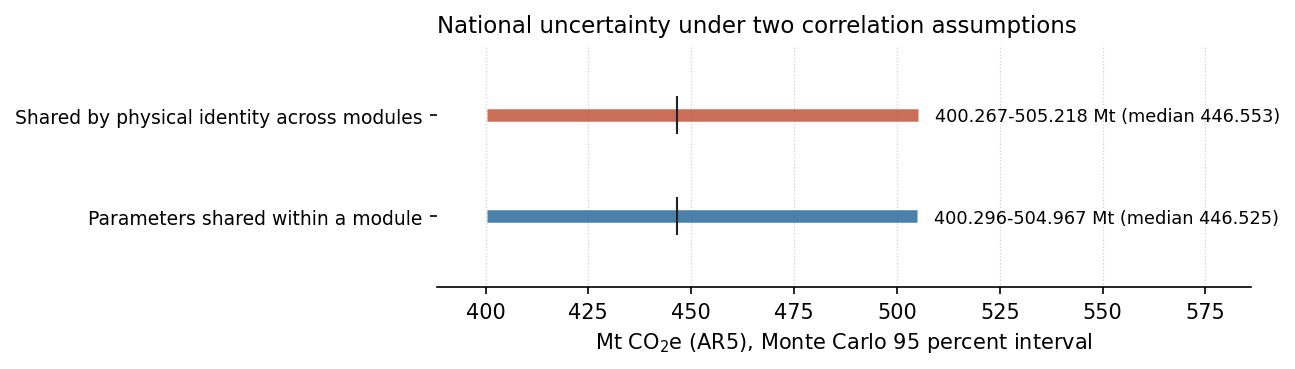
\includegraphics[width=\linewidth]{fig_uncertainty.png}
\caption{95 percent Monte-Carlo intervals for the national total (2.5th to 97.5th
percentile, median ticked) under the two correlation assumptions. The two bars are nearly
identical, which is the finding. Sharing a physical factor prevents the contribution of
that factor from averaging independently across the rows that use it, while preserving each
row's other activity, conversion and residual uncertainties.}
\label{fig:uncertainty}
\end{figure}

\subsection{Reading the gap}

Three things follow, and the first is a correction to what this paper previously reported.

\textbf{At the national level the effect is below the reporting precision:
$\pm\SI{11.72}{\percent}$ either way.} An earlier edition put every fossil-CO\textsubscript{2} component
of every fuel-burning module into ONE correlation group and reported the national band
widening by a fifth. That grouping is not a physical claim. It asserts that the IPCC carbon
contents for diesel, petrol, natural gas, coal, furnace oil and jet kerosene are all wrong
together, in the same direction, by the same relative amount. Grouped per factor---which is
what the shared-default argument actually supports---the eight factor groups are independent
of one another, their variances add in quadrature, and the national effect largely cancels.
The finding as previously stated was an artefact of the grouping.

One coupling was, however, genuinely missing rather than over-asserted, and closing it
is what brought the two scenarios onto the same reported figure. Urea \COtwo{} is
\emph{derived} from the audited national nitrogen offtake---the same series that drives
the synthetic-fertiliser soil pathways---yet the scope registry named that one series
twice, once per receiving category, so a draw moved managed soils and urea application
independently. No physical reading supports that: if the national offtake is wrong, it
is wrong for both. Scoping it as one parameter across both categories is that change, and it widens the
agriculture band by about a hundredth of a percentage point---the direction the
supplement predicted, at a magnitude far below what any reader should act on.

\textbf{At parameter level the effect becomes negligible and is indistinguishable from
Monte Carlo sampling noise at the reported precision.} The
transport module reads $\pm\SI{12.93}{\percent}$ under both correlation structures and the
road-transport category from $\pm\SI{13.26}{\percent}$ to $\pm\SI{13.24}{\percent}$---a
movement smaller than the batch-means standard error published beside its band. The earlier edition reported the road
category widening from \SI{11.96}{} to \SI{18.46}{\percent} on this assumption, and that was
an artefact of the model rather than a property of the inventory: a component could carry only
ONE correlation group, so putting a row in the fuel-carbon group made its \emph{entire}
variance move with the factor. The carbon content of diesel carries about \SI{2}{\percent};
a road class row carries thirty to sixty. Correlating two points of a fifty-point variance
across rows cannot widen their sum, and once the row's activity, conversion and factor are
carried separately it does not.

\emph{The road-transport band is wider than the previous edition published}---\SI{13.3}{}
against \SI{12.0}{\percent}---and that is the same correction seen from the other side. The
OCAC Road control is genuinely one quantity behind every class row, and the old model had no
way to say so while the fuel factor occupied the row's only correlation slot.

\textbf{Once uncertainty is decomposed by parameter, cross-module sharing of the same
physical fuel-carbon factors has a negligible effect on both national and transport
intervals.} The earlier large effect was created by moving the whole component variance with
a factor representing only a small portion of that variance. The argument for publishing the
correlation model beside every band survives the correction: the two scenarios answer
different questions, and only reporting both shows that the answer no longer depends on
which one is asked.

The correlated case is a \emph{bound}, not a better estimate. Perfect correlation is as
strong an assumption as perfect independence, and the truth is between them: the six modules
do share an IPCC default, but they burn physically different fuel batches with genuinely
different carbon contents, and their activity uncertainties remain independent. We report
both endpoints and choose neither, on the same principle applied to the waste sector's
disputed methane correction factor. The honest statement is that the national uncertainty is
$-\SI{10.3}{\percent}/+\SI{13.1}{\percent}$ about the median (symmetric summary
\SI{11.8}{\percent}; $-\SI{10.0}{\percent}/+\SI{13.5}{\percent}$ about the
deterministic reference) under either assumption, and that what the assumption is worth at
national scale is now smaller than the Monte Carlo noise on the estimate.

\textbf{What this exercise is, and what it is not.} It is a \emph{declared covariance
sensitivity}: two named dependency assumptions, run and reported, with the difference between
them attributable to the assumption. It is not an estimate of the true covariance structure of
the underlying activities and factors, and it should not be read as a confidence bound on that
structure.

What the two scenarios vary is \emph{where sharing stops}. A component's draw is the product
of one multiplier per named parameter that enters it and a residual multiplier private to the
row, so a power gas row draws the TOE-to-terajoule conversion, the IPCC carbon content of
natural gas and its own metered activity as three separate quantities. Under the
within-module scope every parameter is qualified by its module, so the carbon content of
diesel is treated as a different quantity in railways and in road transport---which is what an
inventory compiled sector by sector implicitly assumes. Under the cross-module scope it is one
quantity everywhere.

An earlier edition of this machinery gave each component a single correlation group. That
forced a choice between a row's conversion and its factor, and excluded the power module from
the fuel-carbon scenario altogether because its rows were already spoken for by the TOE group.
That limitation is gone. The one that remains is coverage rather than architecture: a
parameter can be shared only once it has been named, and the registry does not yet name every
quantity behind every row. Section~\ref{sec:paramcoverage} reports how far it reaches.

\subsection{Parameter coverage, and what the variance is attributed to}
\label{sec:paramcoverage}

Sharing parameters requires naming them, so the natural question is how much of the inventory
the registry reaches. The answer should be read as a statement about the registry rather than
about the physics.

Of the \num{202} component rows, \num{202} carry at least one named parameter and \num{200}
carry more than one---the case the previous machinery could not express at all. The registry
holds \num{672} parameters; \num{141} dependency groups carry variance in the published run,
and 92 of those enter more than one row, which is what makes correlation possible at
all. The largest single addition is agriculture's factor table
(\texttt{outputs/agriculture\_uncertainty\_inputs\_2024.csv}): the sector composed its IPCC
factor uncertainties inside each row's declared width, where the registry could not see
them, and naming them---the same values, the same widths, no new numbers---is what
brought them inside it. Each row's marginal is decomposed as a sum over its named parameters plus a residual:
where the declared row width covers its parameters, the residual closes the identity exactly
and the marginal is the declared one; where the named parameters imply \emph{more} variance
than the row declares, the parameter graph is authoritative---the marginal is derived from
the parameters under a per-row disposition in
\texttt{data/uncertainty\_reconciliation.csv}, and the declared width is published beside it
as a comparator. The audit register carries \num{59} dispositioned rows: the original
twenty-three were rows a previous edition clamped silently, and the audit found most of
them one resolver defect (a median summarising a multi-member group with another row's
width); after its repair \num{37} rows remain derived at the reference year, each carrying
a named cause---a declared width that omits terms the sector's own input table carries, or
a sector width propagated through a nonlinear model the linear quadrature legitimately
disagrees with. Seven of the dispositions are the naming's own find: HISTORICAL panel
years compose the FAOSTAT projection's activity widths while the registry holds the census
year's, so those rows derive from the graph in the panel years and reconcile exactly at
the reference---the vintage difference published, not clamped. The twelve newest are the
manure and managed-soils N$_2$O rows: once the herd and crop draws were scoped to the
streams they physically drive, their declared widths---the emission factor's alone---were
found to omit the activity the engine multiplies in, and the graph now carries them at
\SIrange{107}{124}{\percent} against the \SIrange{101}{114}{\percent} they declared.

Which quantities drive the national uncertainty is read from the released ensemble itself,
not from a decomposition fitted to it. \texttt{outputs/pakemis\_uncertainty\_drivers.csv}
gives each category's and each module's share of the variance of the national total across
the \num{10000} released draws---the covariance of the category with the total over the
variance of the total, so the shares sum to one---its share of the excess in the top and
bottom 2.5 per cent of draws, and the national interval with that one category held at its
deterministic value. Enteric fermentation carries \SI{59.8}{\percent} of the variance,
managed soils \SI{14.0}{\percent}, domestic wastewater \SI{9.0}{\percent}, manure
management \SI{5.6}{\percent} and rice cultivation \SI{4.0}{\percent}; by module,
agriculture carries \SI{83.5}{\percent} and waste \SI{11.1}{\percent}. The upper tail has
the same order: of the excess in the top 2.5 per cent of draws, enteric fermentation is
\SI{60.1}{\percent}, managed soils \SI{14.7}{\percent} and domestic wastewater
\SI{10.5}{\percent}. With enteric fermentation held fixed the national interval narrows
from \SIrange{399.8}{505.4}{\mega\tonne} to \SIrange{420.3}{483.9}{\mega\tonne}.

The product carries one parameter row. The wastewater effluent factor, frozen at its
default in a rerun of the waste engine on the same draws, carries \SI{4.1}{\percent} of the
national variance and \SI{4.8}{\percent} of the upper tail. Parameter-level importance is
not otherwise claimed. Earlier editions ranked named parameters by Sobol indices estimated
on a surrogate of the simulation; that decomposition, its estimator sweep and its
convergence table are retired, with every figure drawn from them.

\subsection{What the interval leaves out}
\label{sec:bridge}

The interval above is \emph{conditional on one structural configuration}, and that
configuration is larger than any one axis of it. The residential dung basis is a single
axis---which reading of the dung evidence the residential sector takes, the household survey in the reference---while the
\SI{444.96}{\mega\tonne} total rests on \num{23} such choices, of which it is one. Configuration~L, the alternative on that axis, is a first-class key rather than a delta: the annual product carries its residential rows under \texttt{configuration\_id}, beside the reference's typed dung residual, its spatial products are gridded through the same dispatch as the reference: \texttt{pakemis\_grid\_0p05\_monthly\_ledger.nc}, \texttt{pakemis\_adm1\_ledger\_2024.csv} and \texttt{pakemis\_adm2\_ledger\_2024.csv} at stream~$\times$~gas~$\times$~month, differing from the reference in the two dung-cake streams' masses and in no other cell, and \texttt{pakemis\_ensemble\_ledger\_summary.csv} prices it on the same \texttt{draw\_id} as the reference ensemble, so the configuration delta is a per-draw difference rather than two unrelated intervals. They are recorded as a scenario
registry, \texttt{REF\_2023\_24} in \texttt{data/scenarios.csv}, and the release manifest
carries the whole object rather than the letter.

Figure~\ref{fig:bridge} prices each published alternative and draws the one unpriced axis as a labelled empty slot; \texttt{outputs/national\_axis\_register.csv} is the definitive one-row-per-axis table (family, reference setting, deltas, pricing status, and the reason where unpriced). The coal energy basis in
power is worth \SI{1.6}{\mega\tonne}, the sewer methane correction factor
\SI{9.1}{\mega\tonne}, and the fugitive practice assumption \SI{8.6}{\mega\tonne}. Each of
those is \emph{smaller} than the parametric interval, which is about \SI{52}{\mega\tonne} at
the 95th percentile---and \emph{none of them is inside it}. That is the point, and it is not
the same point as being larger: the interval is conditional on the reference configuration and
does not vary these axes at all, so their effect is not represented in it at any width. A
reader given only $\pm\SI{11.7}{\percent}$ has no way to see that they exist.

\begin{figure}[htbp]
\centering
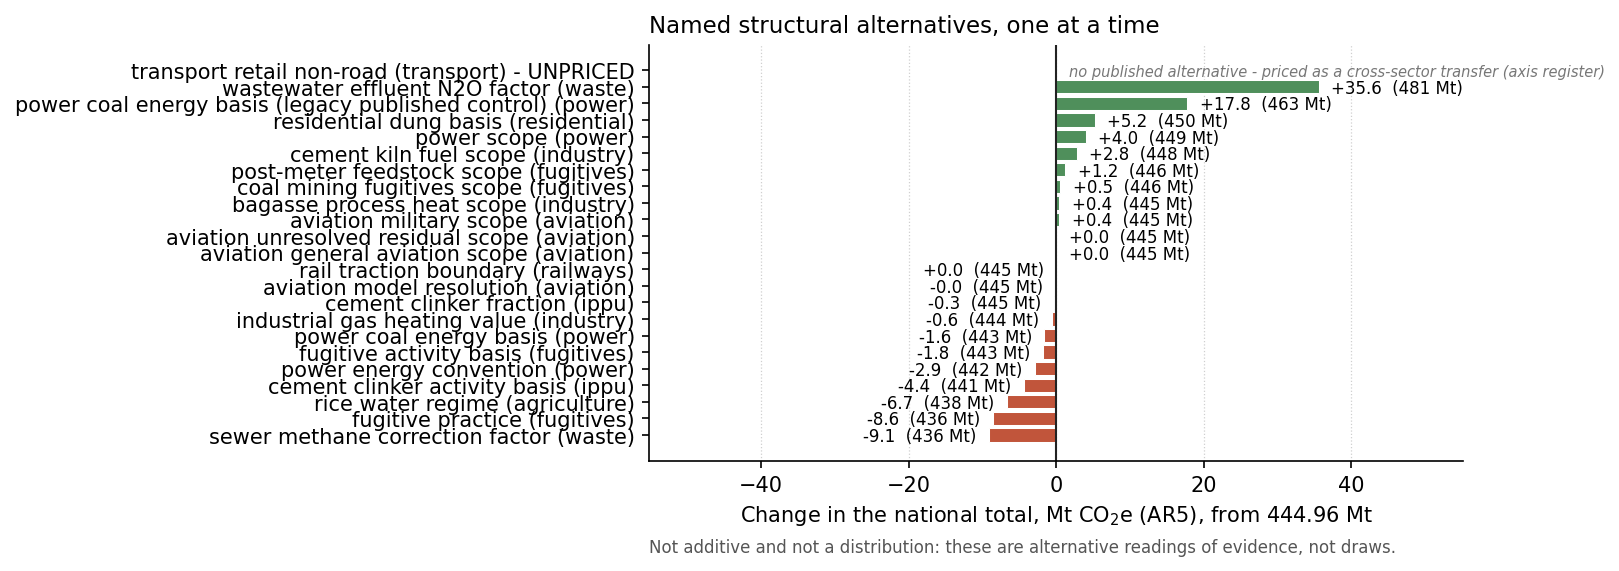
\includegraphics[width=\linewidth]{national_structural_bridge.png}
\caption{The deterministic effect of each named structural alternative on the national total,
one at a time, from \texttt{outputs/national\_structural\_bridge.csv}. \textbf{The bars are not
additive and are not a distribution.} Two of the power axes describe the same coal energy in
different ways and cannot both be taken; none carries a probability, because assigning one
would be the fiat this inventory declines. The transport retail non-road axis has no
single published alternative and is priced as a cross-sector
transfer in the transport supplement instead.}
\label{fig:bridge}
\end{figure}

The same pricing ships in a second, policy-facing form:
\texttt{outputs/national\_configurations.csv} names nineteen single-axis
configurations---the reference, seventeen alternatives a policy reader would ask for by
name (the aviation scope fork ships as three of them: military
attribution, general-aviation activity and the bridge's unresolved residual are
separate evidence questions, priced separately; the post-meter feedstock scope returns
fertilizer feedstock to the leak base, the membership of every release through rc66, retained
and not defended, and the newest is the power coal
calorific basis, which asks the coal-energy question a second way with no heat
rate anywhere in it and so, unlike the member beside it, does not divide the
generation back out of an energy that contains it), and one reporting recode whose
delta is zero by construction---each the scenario
with exactly one axis moved to its published alternative
reading, resolved through the same machinery as the bridge so the two products cannot
disagree. Eight further rows are declared exceptions to the one-axis rule, each
labelled as the exception it is: the fugitives envelope floor (seven axes at their
minimal legs at once), the cross-sector gas deduction (a net-of-leakage adjustment
no single module's scenario table can carry), the central practice reading
(a third reading of the fugitive-practice control, which the one-alternative-per-axis
registry schema cannot hold), and the five scope screenings whose categories sit
outside every module's own scenario table---the F-gas consumption bound, the
commercial/institutional floor, nitric acid unabated and at its last verified
abatement, and the ammonia gas-balance ceiling. The reference now books the stations' own metered coal at IPCC rank defaults, so the
members of this family describe the accounts it replaced. If the coal energy is instead
taken at the calorific values the plants' own generation implies---the heat-rate route,
whose energy contains the generation it is later divided by---the total is
\SI{443.4}{\mega\tonne} (\emph{power\_plant\_physical\_coal}); on NEPRA Table 3's
published conversion, the reference for every release before the coal re-base and retained
as a named control because it implies net fleet efficiencies outside 28--47 per cent in
seven of nine years---it is \SI{462.7}{\mega\tonne}
(\emph{power\_table3\_legacy\_control}); if the Tier~1
clinker model at the 0.75 fraction were taken in place of the producer census, it is
\SI{440.5}{\mega\tonne} (\emph{cement\_tier1\_model\_low}); with the K-Electric system's fuel added to
the power boundary it is \SI{449.0}{\mega\tonne} (\emph{power\_with\_kelectric}), a coverage
alternative priced beside the reference and not added to it: whether the national fuel
statistic already contains K-Electric's fuel is not established, and if it does, adding it
would count that fuel twice.

The file also carries a structural grouping: the power alternatives and the reference are
labelled ONE FAMILY (\texttt{family\_id} \texttt{power\_grid\_control}), because they are
competing definitions of the same grid control---38.45, 40.04, 44.05 and
\SI{57.82}{\mega\tonne} at the sector level---rather than independent axes. They are not
alternatives of one kind, and the file's \texttt{family\_kind} column says which each is:
38.45 is a fuel-property alternative on the reference's own fleet, 44.05 a coverage
alternative that adds the K-Electric system's fuel, and 57.82 a legacy published account
retained for traceability. A range may be formed only within one kind.

\textbf{The selection rule changed with this release, and the previous one rested on an
argument that does not hold.} Every release until now took the regulator's published
national statistic, and the declared reason was that Pakistan's UNFCCC filing agreed with
it on solid fuels to 2\,per cent, which was held to be standing counter-evidence against
the plant-implied coal case. That agreement is not evidence: the filing is compiled from the
same energy balance the regulator reports, so the two agree by provenance, and
\texttt{data/validation\_catalog.csv} has carried that row at independence class
\texttt{none} throughout. The rule now rests on a test neither account can satisfy by
construction. Dividing each candidate coal energy into the regulator's own printed
generation gives an implied net fleet efficiency; against the 28--47\,per cent envelope the
published conversion lands inside in TWO of nine panel years and the generating stations'
own metered coal at IPCC rank default calorific values lands inside in SEVEN, with the
remaining two straddling the envelope rather than falling outside it. Those two are
FY2016--17 and FY2017--18, the years whose commissioning coal is bounded rather than
printed, and the straddle is a property of that interval: it is bounded by the intensity
range the same two stations run at over the ledger years, which includes a sharply
curtailed year, and a commissioning plant is a part-load plant, so the low-intensity end
of that range is the relevant one rather than an outlier to discard. A narrower band
would place the whole interval inside the envelope, and would do so by excluding the most
analogous observation available. Neither side
of that test touches a heat rate, so neither restates the regulator's own print---which the
third candidate, the heat-rate route at \SI{38.45}{\mega\tonne}, does by construction and is
why the re-base did not go there.

The reference is therefore \SI{40.04}{\mega\tonne}, and the conversion it replaced is
retained as \texttt{power\_table3\_legacy\_control} at \SI{57.82}{\mega\tonne} rather than
deleted, so a reader holding a total published before this release can find the account it
came from. It is not equally probable with the reference and the registry says so, which is
also why it is excluded from the priority ranking of unresolved choices. The per-year moves,
and the mass and calorific terms whose product is each year's ratio, are published in
\texttt{outputs/pakemis\_power\_coal\_rebase\_ledger.csv}; the four candidate accounts with
their efficiency verdicts are in
\texttt{outputs/pakemis\_power\_coal\_configurations.csv}. Every quote of the grid figure,
here and in the results section, is conditional on that rule with the alternatives named
beside it; the structural bridge carries the same \texttt{family\_id} tag on its power axes.

One constraint on those candidate explanations is new here and narrows all of them at
once. Each supposes a constant difference between the regulator's two tables---a calorific
convention, a gross basis, a scope, a stock change---and a constant difference has a
constant sign. Across the five years the plant ledger spans it does not.
\texttt{outputs/pakemis\_power\_coal\_energy\_adjudication.csv} divides each energy
figure by the coal generation the regulator itself reports, a test that uses no tonnage and
so cannot be undone by an error in one: Table~3's energy implies a fleet net thermal
efficiency of \SI{57.5}{\percent} in FY2020--21 and \SI{18.9}{\percent} in FY2023--24.
No thermal fleet spans that range, and a plant set that is too wide makes energy too high
in every year rather than too low in one. Over the same years the plant-level route implies
\SIrange{32.4}{45.7}{\percent}, which is a fleet.

The break is dated, and it is not a revision between editions: the 2024 edition prints
FY2018--19 to FY2021--22 side by side in the same table, and the 2025 edition reproduces
those columns exactly. Across two adjacent columns of that one table the coal
tonne-of-oil-equivalent figure rises \SI{87.5}{\percent}, from \num{4123008} to
\num{7731514}~TOE, while the same report's per-station table has coal mass falling
\SI{7.3}{\percent} and coal generation falling \SI{3.5}{\percent}.

It \emph{is} a conversion, and over a panel longer than the plant ledger it is a constant
one. Table~3 states that it takes these figures from the HDIP \emph{Pakistan Energy
Yearbook}, and HDIP's own power-sector coal tonnage is held here as well, republished in the
Economic Survey's statistical supplement. Against \emph{that} tonnage Table~3's energy works
out at \num{0.447} tonnes of oil equivalent per tonne in every year from FY2015--16 to
FY2020--21---six consecutive years spanning \num{0.000072}~TOE per tonne, or
\SI{0.016}{\percent}---and \num{0.604}, \num{0.511}, \num{0.478} thereafter.
\texttt{outputs/pakemis\_power\_reference\_audit.csv} carries the span year by year, and
\texttt{outputs/pakemis\_power\_fuel\_reconciliation.csv} carries the plant, fuel and year
account the constant is measured against: coal mass, rank, generation and the energy they
imply, for all nine years rather than the five the per-station table reaches, with the
edition and table each number was read from and an interval wherever no edition prints a
mass. That
constant is \SI{18.73}{\tera\joule\per\giga\gram}: one generic coal factor, applied whatever
the fleet happened to be burning. It breaks in FY2021--22, and it breaks \emph{upward}---to
\SI{25.27}{}, then \SI{21.40}{} and \SI{20.02}{}---over exactly the years the fleet's own
physical calorific value falls from \SI{20.34}{} to \SI{13.01}{\tera\joule\per\giga\gram} as
Thar lignite scales. A measured energy cannot move the wrong way against its own fuel. An
earlier version of this section read the first two of those six years and concluded the
opposite; the panel simply began too late to see the constant. What \emph{also} moves is the
ratio of the two tonnage accounts: HDIP's national series against the regulator's own per-station
quantities runs \num{0.88}, \num{0.70}, \num{1.05}, \num{1.11}, \num{1.21}, crossing unity
between the two years in question. A scope difference cannot cross unity. A
consumption-against-receipts difference could, in either direction, and nothing held settles
which.

A physical screen then narrows them, though it does not choose between them. Taking each
tonnage account at the fleet's own rank composition---IPCC default calorific values, no heat
rates---and dividing the electricity out of it, the per-station account gives
\SIrange{34.4}{38.7}{\percent} in every one of the five years: a fleet, inside the band
throughout. HDIP's national series gives \SI{49.0}{\percent} falling to \SI{29.1}{\percent},
outside at both ends. Of three accounts of the same coal, one is physically admissible across
the panel and two are not. That screen is a plausibility filter on a candidate energy level
and \emph{not} independent corroboration of the account it favours: the efficiency it reports
is the electricity divided by exactly the energy that route constructs, which is an identity
rather than a comparison, and the audit above recomputes it year by year to show so. It can
reject an energy level as unphysical; it cannot adjudicate between two tonnage accounts that
imply the same energy.

\texttt{outputs/pakemis\_power\_coal\_configurations.csv} states the four candidate coal
accounts year by year with what each depends on, and the column that matters is whether the
calorific value was derived from generation. One of them was: the \SI{38.45}{\mega\tonne}
alternative this paper names beside the reference takes heat-rate-implied calorific values,
so its energy contains the generation it is later divided by and its implied efficiency
restates the regulator's own print rather than testing it. The rank-default route, which
uses no heat rate and is the only candidate independent of the electricity it is judged
against, was published nowhere before that file. Its ratio to the published energy runs from
\num{0.47} to \num{2.00} across the panel and crosses unity twice, and decomposes exactly
into a tonnage term that stays within \numrange{0.74}{0.99} and a calorific term that runs
\numrange{0.63}{1.38}: the sign change is the conversion, which is why no single correction
factor exists. That the composition is
genuinely moving underneath all three is not in doubt: the fleet's lignite share by mass goes
from \SI{27.6}{\percent} in FY2020--21 to \SI{39.3}{\percent} in FY2021--22 and reaches
\SI{92.0}{\percent} by the reference year, which is why a calorific value that rises over
the same span is the wrong shape whatever tonnage it is divided by. A third route, taking the
same tonnages by rank at IPCC default calorific values and no heat rate at all, falls with
the fleet as the plant route does.

None of this overturns the selection. The official reporting filing agrees with the
regulator's coal energy to within \SI{2}{\percent}, which is the standing counter-evidence
the rule already cites, and this inventory continues to take the published national
statistic. What the constraint establishes is narrower and, for a reader deciding how much
weight the \SI{40.04}{\mega\tonne} figure carries---against the \num{38.45},
\num{44.05} and \num{57.82} alternatives named beside it throughout---more useful: whichever reading is
right, it is not one that holds constant across the panel, so the open question is not only
\emph{which} table to believe but \emph{when} its basis changed.
No probability attaches to any row---the schema forbids the column---and the rows do
not compose: each is one axis off the reference, not a corner of a scenario space.

One axis carries a finer question than its name, and it gets its own table. Under
the reference the household survey observes \SI{10.93}{\mega\tonne} of dung cake against
the ledger's \SI{58.74}{\mega\tonne} diversion, and mass conservation cannot say where the
other \SI{47.81}{\mega\tonne} went---conservation proves the mass exists, not its
destination. But the candidate destinations are not interchangeable: each has different
\CHfour{}, \NtwoO{} and biogenic-\COtwo{} consequences, so the survey reading alone under-describes the
national reading. Table~\ref{tab:dungvariants} prices each destination declared in
\texttt{data/scenario\_variants.csv}, with no probabilities. The non-household-combustion
variant lands on the L~total exactly, because the residual burning anywhere on the same
fuel chain emits what L counts---a reclassification, not a new quantity---and that
equality is asserted by test rather than observed. The survey reading carries its own
uncertainty, and the reference prices it: the dung stream is drawn at \SI{35}{\percent}
activity uncertainty, the width firewood carries.

\begin{table}[htbp]
\centering
\footnotesize
\begin{tabular}{@{}p{0.46\linewidth}rr@{}}
\toprule
\textbf{Destination of the 47.81 Mt residual} & \textbf{$\Delta$ vs reference} & \textbf{National} \\
\midrule
Declared unresolved stock (the reference) &  0.00 & 444.96 \\
Non-household combustion, same fuel chain & 5.25 & 450.20 \\
Return to manure management               & 4.49 & 449.44 \\
Field application (soils \NtwoO{})        & 3.49 & 448.44 \\
Diversion fraction revised down           & 4.49 & 449.44 \\
\bottomrule
\end{tabular}
\caption{National consequences of each destination for the reference's unresolved dung
residual, Mt \COe{} (AR5), from \texttt{outputs/national\_dung\_variants.csv}. Every
variant conserves the diverted mass exactly (asserted at write time); none carries a
probability. Return-to-manure and revised-diversion price identically because the
arithmetic is the same---what differs is which reading of the evidence is being revised,
and the published note says so. The residual is worth between \num{3.5} and
\SI{5.2}{\mega\tonne} depending on where it went, which is why conservation alone cannot
close the scenario.}
\label{tab:dungvariants}
\end{table}

\subsection{One ensemble, joinable: the common draw\_id}
\label{sec:ensemble}

Until this release, every uncertainty product answered its own question in its own file
and nothing shared a draw: the annual Monte Carlo published percentiles, the monthly
layer carried deterministic brackets, the spatial products carried none by declared
design. A reader could not ask ``in the realisations where the national total is high,
which months and which provinces are high?''---and the two closure identities the
deterministic products enforce at $10^{-9}$ were not even \emph{expressible} per draw.
The common ensemble makes them expressible and then asserts them inside every one of its
\num{10000} draws: \texttt{outputs/mc\_draws/pakemis\_ensemble\_\{annual,monthly,%
spatial\}.parquet}, joined by a single \texttt{draw\_id}, with
$\sum_{m=1}^{12} E(d,c,m) = E_{\mathrm{annual}}(d,c)$ and
$\sum_{\mathrm{prov}} E(d,c,p) + E_{\mathrm{retained}}(d,c) = E_{\mathrm{annual}}(d,c)$
holding to $10^{-9}$ in every draw $d$ (the second is the gridded-plus-unallocated
identity, carried as a placement axis). Every stream in the national pool is
identity-seeded, so draw $d$ of the ensemble is \emph{bit-identically} draw $d$ of the
published \num{100000}-draw run---a prefix given a name, not a second simulation---and a
test asserts the bit-identity. The summary surface
(\texttt{outputs/pakemis\_ensemble\_summary.csv}) publishes each grain's quantiles with
batch standard errors beside the published run's, which is the convergence statement for
the prefix.

What is drawn and what is not follows the evidence, per category and stated in a column.
Monthly profile weights are \emph{drawn} only where a measured dispersion exists---the
hindcast WAPE streams, road transport and railways, whose weights take multiplicative
noise sized by the measured error and renormalise to sum to one inside every draw---and
are degenerate everywhere else
(\texttt{profile\_uncertainty\_status}); the power fuel-mix variant remains a conditional
configuration and is never mixed in. Spatial shares are fixed per draw---allocation is
declared, not sampled---so the spatial layer's per-draw variation is the parametric mass
reaching each province, and the priced allocation alternatives ship as conditional
quantile blocks over the same draw\_ids
(\texttt{outputs/pakemis\_ensemble\_spatial\_conditionals.csv}), never as a mixture. A
month-by-cell ensemble would be roughly \num{118} gigabytes and is deliberately absent:
the ensemble is marginal by design, category grain for months and province grain for
space, and the deterministic weights whose sums-to-one the cube gates already enforce
carry each draw the rest of the way. The five kinds of uncertainty this release
separates---parameter, profile, placement, structure, completeness---each have a carrier
product and an aggregation rule, stated in \texttt{docs/uncertainty\_contract.md}; the
completeness kind rides the joint lattice as a bound
(\texttt{completeness\_bound\_Mt}) beside the interval, never a distribution inside it.

Structure gains a time axis the same honest way. The twenty-two registered axes were priced
against the reference year only;
\texttt{outputs/pakemis\_structural\_trajectories.csv} now re-prices each axis in each of
the nine panel years where its engine honestly can---92 axis-years priced on their
own years' activity---and refuses the rest with the missing evidence named per row
(93 refusals; the producer
census that is own-year by construction, the scenario runners that price the reference
year only). A refusal is a row, never a silence, and no probability attaches to any
point: these are deterministic forks re-read per year, not a trajectory ensemble, and the
longitudinal product's refusal to cross structural axes into a probabilistic ensemble
stands.

\subsection{Where the uncertainty actually lives}

The national band is much narrower than most of its sectors'---\SI{10.9}{\percent} against
waste's \SI{51.1}{\percent} and fugitives' \SI{37.7}{\percent}---which is the ordinary
behaviour of partly independent errors in a sum. Fugitives now contribute
\SI{5.3}{\percent} of emissions and \SI{3.3}{\percent} of Approach-1 variance. Its discrete
practice and coverage scenarios remain outside the pooled Monte Carlo, so the national
probability interval should not be read as absorbing that structural envelope.

The same caveat now applies to electricity generation, whose uncertainty was rebuilt
around its evidence classes: its parametric band fell to $\pm\SI{8.3}{\percent}$ (per-fuel
activity widths, correlated through the shared TOE conversion) precisely because its
one-sided questions---the coal calorific conversion (worth \SI{1.6}{\mega\tonne}), the
TOE gross/net basis, and K-Electric coverage---moved into named structural cases with
conditional intervals and no probabilities. The national interval absorbs none of them,
and the power sector's scenario table is where a reader finds what they are worth.

\subsection{What to measure next depends on the question}
\label{sec:priorities}

The driver shares above answer one of three different priority questions this inventory
publishes, and they are not
interchangeable. Which \emph{category} would most narrow the conditional interval is
a parametric question, and its answer is enteric fermentation, read from the ensemble at
category grain with no ranking of named parameters. The other two are published together
(\texttt{outputs/national\_priority\_rankings.csv}). Which \emph{unresolved model
choice} most moves the deterministic total is a structural question the interval cannot
see, and its answer is the power coal energy basis at \SI{9.1}{\mega\tonne}. Which
\emph{missing category} most changes completeness is a coverage question neither of the
first two can express, and its answer is industrial solid fuel:
EDGAR carries \SI{19.4}{\mega\tonne} for 1.A.2 that this inventory does not estimate.
Reading any one of the three as the measurement priority list silently answers the other
two questions with it.

\subsection{Nine years, and whether their differences are resolved}
\label{sec:longitudinal}

Everything above conditions on the reference year. The nine-year panel is the product a
reader is most likely to difference, and until now it carried no interval at all---so the
only bound available for a year-on-year change was the national
\SIrange{-10.4}{16.0}{\percent}, which is a statement about a \emph{level} and does not
apply to a \emph{change}. \texttt{outputs/pakemis\_longitudinal\_uncertainty.csv} gives every
fiscal year a band and \texttt{outputs/pakemis\_trend\_uncertainty.csv} gives every
consecutive pair and the full window one, differenced draw by draw so that shared error
cancels as the real quantity does.

How much of it cancels is not something the evidence settles, so three correlation scenarios
are published rather than one. At one extreme every component's error is a single draw shared
by all nine years; at the other every error is redrawn wherever the underlying number moved.
The reported scenario is neither: it is typed from the parameter graph, sharing across years
what names a factor, a physical constant or a held parameter, and redrawing what names a
quantity measured in a particular year. Whether a quantity ``moved'' is decided by equality
in-process and enters a stream's seed as the first fiscal year that carries the value, never
as the value's own digits: a one-ulp platform difference in a computed number therefore cannot
re-seed a stream, and the first \num{200} draws of every stream ship as
\texttt{outputs/pakemis\_longitudinal\_prefix.csv} so that a rerun elsewhere is compared with
what this release drew rather than trusted.

\textbf{The resolution statement, read from the product's own rows with scenario and
scope named on every number.} Under the reported (typed) scenario, \num{2} of the \num{8}
consecutive year-on-year changes in the panel are resolved at \SI{95}{\percent}. The
decadal window IS: since the FY2015--16 recovery the panel has one window rather than
two---the common-scope span and the full panel coincide at ten comparable sectors---and
the FY2015--16 to FY2023--24 change of \SI{51.12}{\mega\tonne} resolves at
\SIrange{15.94}{89.57}{\mega\tonne} under the typed scenario and at
\SIrange{40.08}{64.04}{\mega\tonne} under time correlation, but NOT under the
deliberately-widest reading, full time independence
(\SIrange{-10.01}{114.07}{\mega\tonne}), which spans zero.

\textbf{That is a retreat from what this paragraph said before the coal re-base, and the
retreat is the honest reading.} It said that no end of the bracket left the decadal change
spanning zero any more. That was true of the larger change the previous edition
reported and is false of this one under the same intervals. Booking public-power coal on the
generating stations' own metered fuel rather than on the aggregate conversion lowers the
reference year by \SI{17.78}{\mega\tonne} and the FY2015--16 start year by only
\SI{0.19}{\mega\tonne}, so almost the whole move lands on the decadal difference. The
inventory can therefore support a decadal trend statement under two of the three
correlation readings it publishes, cannot support one under the third, and still cannot
resolve a single year-on-year change. A claim that strengthened when the evidence did not
is worth stating as a correction rather than quietly re-scoping.

\textbf{An earlier edition of this section reported one resolved change, and it was an
artefact of a defect in the product beneath it.} The difference table carried a
\texttt{comparable\_sectors} column reporting the sectors two years have in common, while the
arithmetic subtracted every sector present in each year---so any pair reaching back to
FY2015--16, where transport and industry are absent, subtracted eight sectors from ten and
published it under a column saying eight. The one change that appeared resolved was
FY2015--16 to FY2016--17 at \SI{77.92}{\mega\tonne}, of which \SI{61.08}{\mega\tonne} was
two sectors entering the record; restricted to the scope its own column claimed it fell to
\SI{16.83}{\mega\tonne} and stopped resolving, and on the recovered ten-sector panel the
first step is
\SI{25.60}{\mega\tonne} and still not resolved. The full-window figure fell the same way,
from \SI{131.27}{\mega\tonne} to \SI{80.33}{\mega\tonne}---\SI{39}{\percent} of the
headline was the record filling in. Both the point estimate and the draws behind the
interval were restricted to the scope the column claimed, so the band was corrected and
not only the number---and since the FY2015--16 recovery the restriction itself is
history: the published full-panel change is \SI{51.12}{\mega\tonne} over all ten
sectors, like for like.

The reason was measurable, and this release acted on it. The previous edition found
\SI{81}{\percent} of the national variance row-private residual---variance the parameter
graph attributed to no named quantity---and stated that naming parameters, not collecting
more years, was the work that would narrow a trend band. Naming agriculture's factors did
exactly that to the variance composition: \SI{76.56}{\percent} of the reference year's
variance now sits in parameters that persist across years, \SI{20.96}{\percent} in
year-resampling activity, and \SI{2.48}{\percent} in residual. The shares are
covariance-aware: members of one dependency group draw one factor, so their first-order
terms add before they are squared (the previous edition summed the squares and printed
\SI{10.67}{\percent} for the resampling share, half its value). Persistent error is
precisely what a difference cancels, and the cancellation is what resolves the windows
stated above while leaving every consecutive change unresolved---the year steps are small
against the fifth of the variance that resamples each year and the residual that no
parameter names.
